\newcommand{\performerDescription}{
\section{Performer}
\epigraph{\textit{
    "Some people think a club can solve any problem. Unless
    you're a half-giant, there are more sophisticated ways of
    settling a disagreement." } }{ Cabal, half‐elven bard }

    Performers are master the art of entertainment, using their
    performances to amuse nobles and templars and gain wealth.
    Most performers can dazzle a crowd, or incite them to riot.
    Performers tend to learn to play a variety of instruments,
    or recite poetry or old legends by campfire. They can be
    acrobats, performing dazzling displays of physical prowess.\\
    \\
    See \nref{tlttree:performer} for more information.
}

\newcommand{\performerTree}{
    \newpage
    \subsection{Performer Talent Tree}
    \label{tlttree:performer}

    \textbf{Class Skills:} Athletics, Charm, Cool, Coordination, Deception, Streetwise
    \newline

    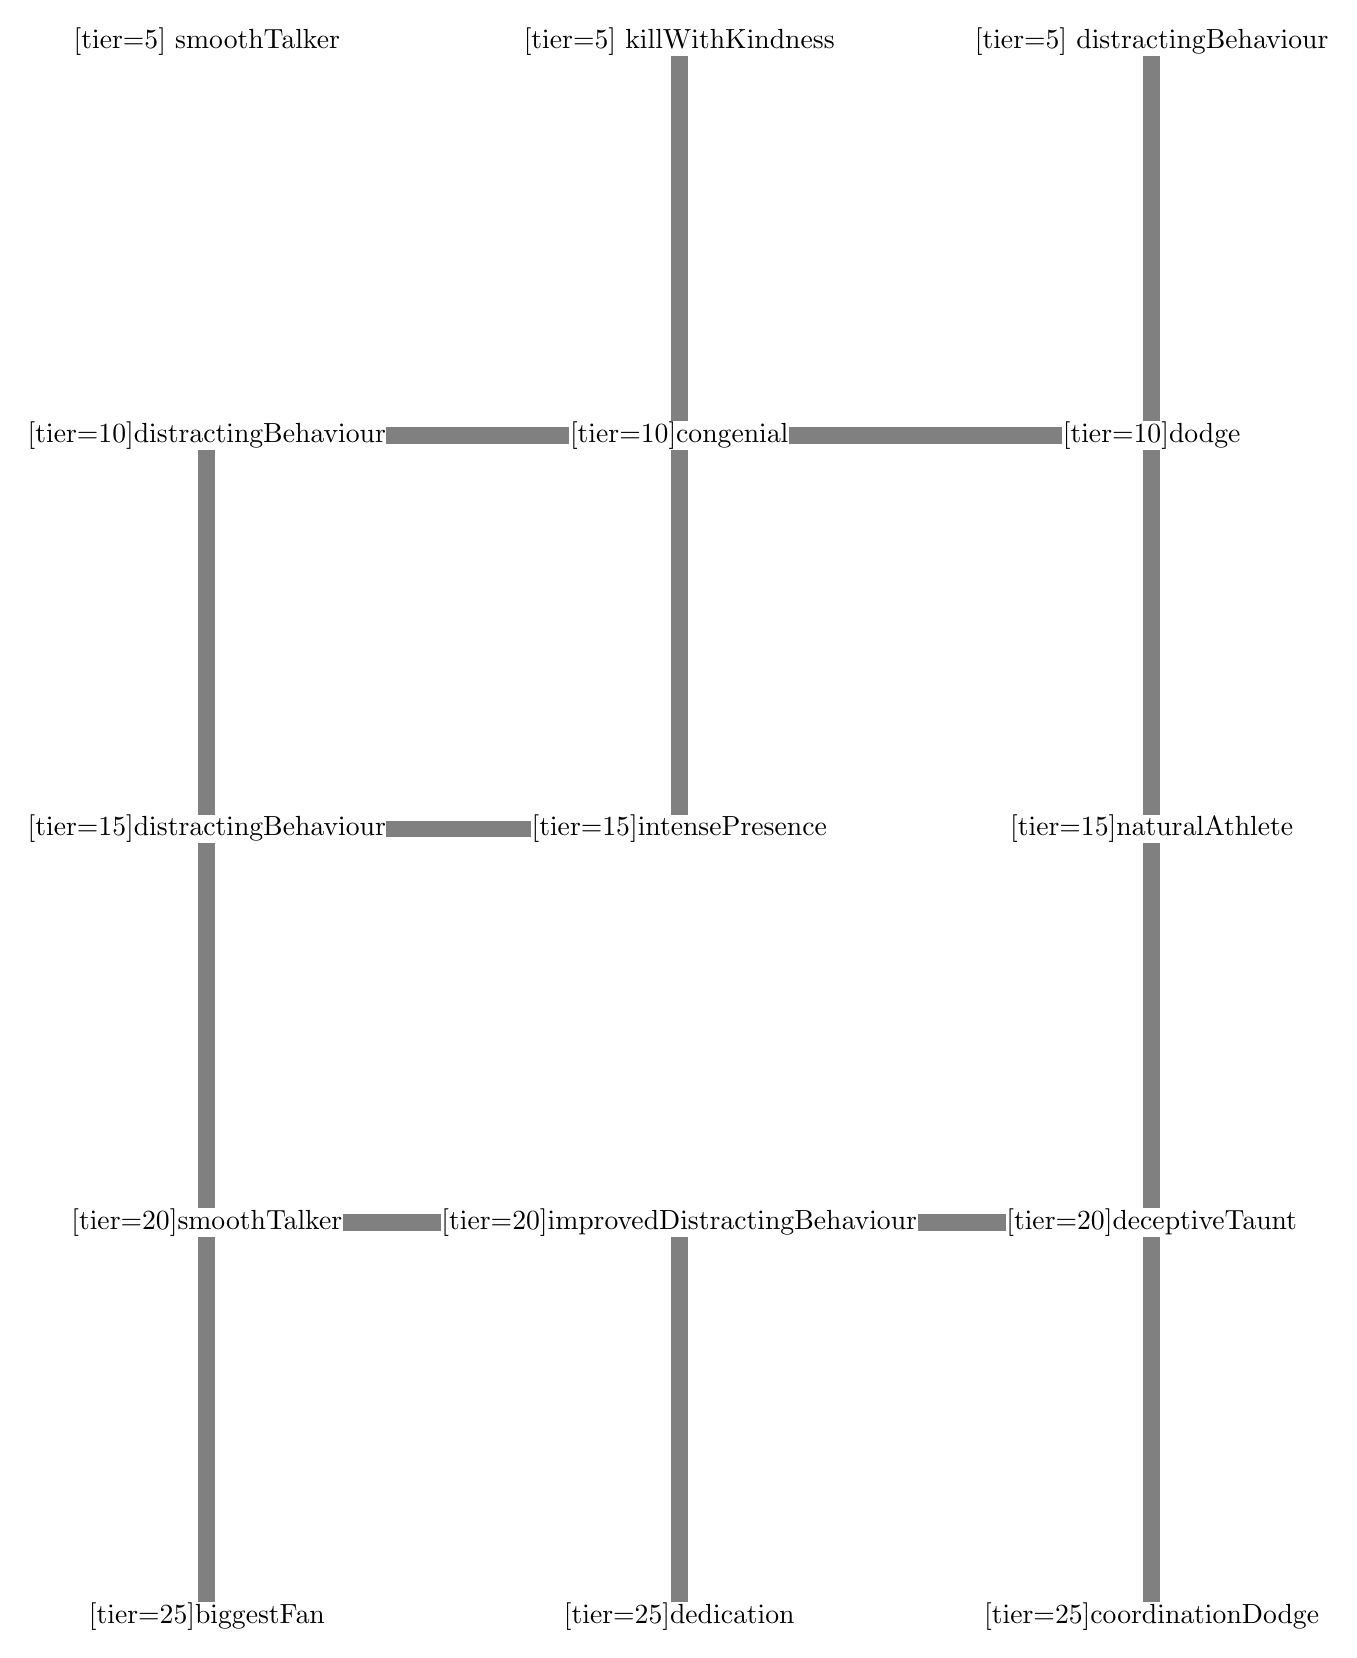
\begin{tikzpicture}
        \draw ( 0,  0) node(aa)[inner sep=0]{\TalentBox[tier=5] {smoothTalker}}
              ( 6,  0) node(ab)[inner sep=0]{\TalentBox[tier=5] {killWithKindness}}
              (12,  0) node(ac)[inner sep=0]{\TalentBox[tier=5] {distractingBehaviour}}
              ( 0, -5) node(ba)[inner sep=0]{\TalentBox[tier=10]{distractingBehaviour}}
              ( 6, -5) node(bb)[inner sep=0]{\TalentBox[tier=10]{congenial}}
              (12, -5) node(bc)[inner sep=0]{\TalentBox[tier=10]{dodge}}
              ( 0,-10) node(ca)[inner sep=0]{\TalentBox[tier=15]{distractingBehaviour}}
              ( 6,-10) node(cb)[inner sep=0]{\TalentBox[tier=15]{intensePresence}}
              (12,-10) node(cc)[inner sep=0]{\TalentBox[tier=15]{naturalAthlete}}
              ( 0,-15) node(da)[inner sep=0]{\TalentBox[tier=20]{smoothTalker}}
              ( 6,-15) node(db)[inner sep=0]{\TalentBox[tier=20]{improvedDistractingBehaviour}}
              (12,-15) node(dc)[inner sep=0]{\TalentBox[tier=20]{deceptiveTaunt}}
              ( 0,-20) node(ea)[inner sep=0]{\TalentBox[tier=25]{biggestFan}}
              ( 6,-20) node(eb)[inner sep=0]{\TalentBox[tier=25]{dedication}}
              (12,-20) node(ec)[inner sep=0]{\TalentBox[tier=25]{coordinationDodge}}
        ;

        \tikzstyle{bar}=[gray,-,>=stealth, line width=6pt]

        \draw [bar] (ab) to (bb);
        \draw [bar] (ac) to (bc);

        \draw [bar] (ba) to (ca);
        \draw [bar] (bb) to (cb);
        \draw [bar] (bc) to (cc);

        \draw [bar] (ca) to (da);
        \draw [bar] (cc) to (dc);

        \draw [bar] (da) to (ea);
        \draw [bar] (db) to (eb);
        \draw [bar] (dc) to (ec);

        \draw [bar] (ba) to (bb);
        \draw [bar] (bc) to (bb);

        \draw [bar] (ca) to (cb);

        \draw [bar] (da) to (db);
        \draw [bar] (dc) to (db);
    \end{tikzpicture}
}
